% Figura: um PRB em um slot, com os 4 símbolos de DM-RS (2, 3, 10, 11): 48 REs.
%   Separada da Figura fig:dmrs-n em 2026-11-04 (antes era a parte (a)).
%   Cores: azul da escala do mapa (#cde2fb claro, #0d366b escuro); sem verde; sem negrito.
\definecolor{dmrsfill}{HTML}{CDE2FB}
\definecolor{winblue}{HTML}{0D366B}
\definecolor{inksec}{HTML}{52514E}
\begin{figure}[htbp]
\caption{Resource elements of one PRB in one slot, with the DM-RS symbols.}
\label{fig:prb-dmrs}
\vspace{4pt} % a classe zera o espaço entre a caption e a figura
\centering
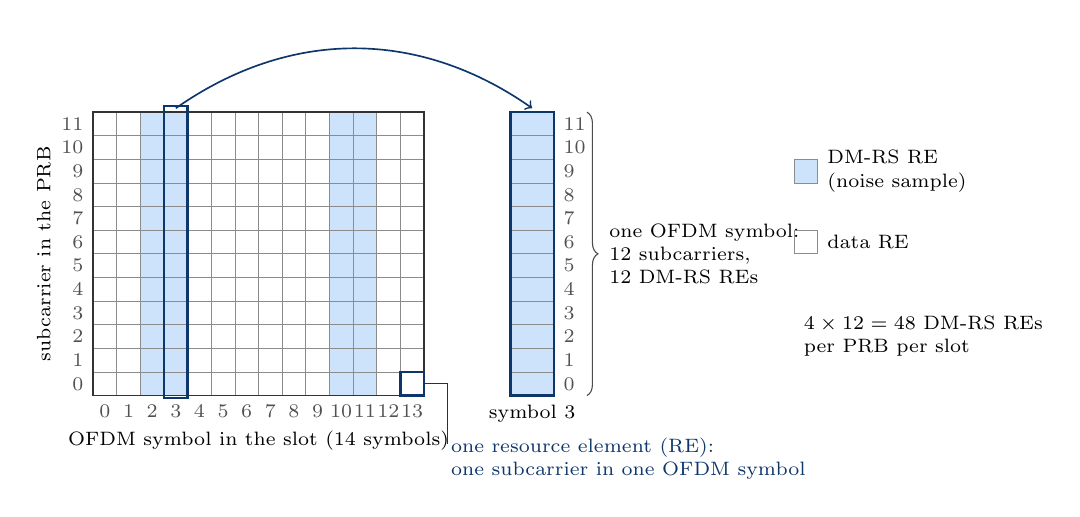
\begin{tikzpicture}[font=\fontsize{7}{8.4}\selectfont]
% ------------------------------------------------------------------ (a)
\def\w{0.30}
\begin{scope}[shift={(0,0)}]
  \foreach \s in {2,3,10,11}
    \fill[dmrsfill] (\s*\w,0) rectangle ++(\w,12*\w);
  \foreach \s in {0,...,14}
    \draw[black!45, line width=0.3pt] (\s*\w,0) -- (\s*\w,12*\w);
  \foreach \k in {0,...,12}
    \draw[black!45, line width=0.3pt] (0,\k*\w) -- (14*\w,\k*\w);
  \draw[black!80, line width=0.6pt] (0,0) rectangle (14*\w,12*\w);
  \foreach \s in {0,...,13}
    \node[inksec, below] at (\s*\w+\w/2,0) {\s};
  \node[below] at (7*\w,-0.32) {OFDM symbol in the slot (14 symbols)};
  % subportadoras numeradas de 1 a 12 (de baixo para cima)
  \foreach \k [evaluate=\k as \kk using int(\k)] in {0,...,11}
    \node[inksec, left] at (0,\k*\w+\w/2) {\kk};
  \node[rotate=90, above] at (-0.42,6*\w) {subcarrier in the PRB};
  % coluna destacada (símbolo 3) e ampliação ao lado
  \draw[winblue, line width=0.9pt] (3*\w,-0.03) rectangle (4*\w,12*\w+0.08);
  \def\zx{5.3}
  \def\zw{0.55}
  \fill[dmrsfill] (\zx,0) rectangle ++(\zw,12*\w);
  \foreach \k in {0,...,12}
    \draw[black!45, line width=0.3pt] (\zx,\k*\w) -- ++(\zw,0);
  \draw[winblue, line width=0.8pt] (\zx,0) rectangle ++(\zw,12*\w);
  \foreach \k [evaluate=\k as \kk using int(\k)] in {0,...,11}
    \node[inksec, right] at (\zx+\zw,\k*\w+\w/2) {\kk};
  \draw[winblue, ->, line width=0.6pt] (3.5*\w,12*\w+0.05) to[out=35, in=145] (\zx+\zw/2,12*\w+0.05);
  \node[below, align=center] at (\zx+\zw/2,0) {symbol 3};
  \draw[decorate, decoration={brace, amplitude=4pt}, black!70]
    (\zx+\zw+0.42,12*\w) -- (\zx+\zw+0.42,0);
  \node[right, align=left] at (\zx+\zw+0.58,6*\w) {one OFDM symbol:\\12 subcarriers,\\12 DM-RS REs};
  % um RE destacado (símbolo 13, subportadora 0), com chamada
  \draw[winblue, line width=0.9pt] (13*\w,0) rectangle ++(\w,\w);
  \draw[winblue, line width=0.5pt] (14*\w,\w/2) -- (14*\w+0.3,\w/2) -- (14*\w+0.3,-0.62);
  \node[winblue, right, align=left] at (14*\w+0.22,-0.80) {one resource element (RE):\\one subcarrier in one OFDM symbol};
  % legenda
  \def\lx{8.9}
  \fill[dmrsfill] (\lx,9*\w) rectangle ++(\w,\w);
  \draw[black!45, line width=0.3pt] (\lx,9*\w) rectangle ++(\w,\w);
  \node[right, align=left] at (\lx+\w,9.5*\w) {DM-RS RE\\(noise sample)};
  \draw[black!45, line width=0.3pt] (\lx,6*\w) rectangle ++(\w,\w);
  \node[right, align=left] at (\lx+\w,6.5*\w) {data RE};
  \node[right, align=left] at (\lx,2.5*\w) {$4 \times 12 = 48$ DM-RS REs\\per PRB per slot};
\end{scope}
\end{tikzpicture}
\vspace{4pt}
\legend{Source: the author, with the DM-RS positions of \citesp{3gpp-ts38211}. \textcolor{red}{Double-symbol DM-RS}, mapping type~A, symbols 2, 3, 10 and 11.}
\end{figure}
